% generated by plots/fig7_targets.py --- do not edit the numbers by hand
% figure* --- the chapter is two-column and this does not fit one
\begin{figure*}[tp]
\centering
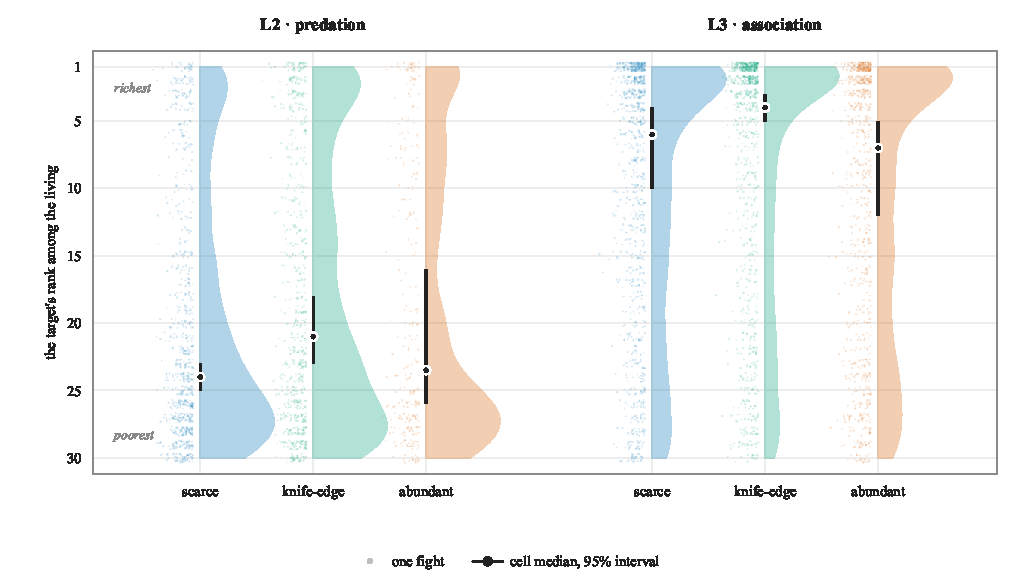
\includegraphics[width=\linewidth]{figures/fig7_targets/target_rank.pdf}\\[2pt]
\caption[Where in the wealth ordering the blows land]{%
\textbf{Where in the wealth ordering the blows land.} Every resolved fight placed at the rank its target held going into the round, richest at the top: 1,923 fights at L2 and 2,928 at L3. Each cell is one object: the points on the left are the fights themselves, the shape on the right is their density, and the dot and bar on the spine are the cell median with a 95 per cent interval on it\meth{m:whom-hit-over}. Random targeting would draw a shape of even width from top to bottom and put the median at rank 15.5.}
\label{fig:targets}
\end{figure*}
